%*****************************************
\chapter{Survey Research}\label{08:surveys}
%*****************************************

\begin{wrapfigure}{R}{0.4\textwidth}
	\label{08:fig01} 
	\centering
	
\includegraphics[width=0.4\textwidth]{gfx/08-01} 
\end{wrapfigure}

How do retailers know what sorts of products their customers are likely to purchase? They use surveys to ask questions. Unfortunately, creating an unbiased survey that asks the right questions is a much more complex task than it may seem. This chapter introduces the art and science of survey design, from types of surveys, writing questions, and analyzing the results.
\blfootnote{Photo by Joshua Rawson-Harris on Unsplash}

\begin{center}
	\begin{objbox}{Objectives}
		\begin{itemize}
			\setlength{\itemsep}{0pt}
			\setlength{\parskip}{0pt}
			\setlength{\parsep}{0pt}
			
			\item Differentiate between cross-sectional and longitudinal surveys
			\item Compare and contrast the four types of longitudinal surveys: trend, panel, cohort, and retrospective
			\item Describe the characteristics of effective questions
			\item Define the various question response options
			\item Describe tips for creating good questionnaires
			\item Discuss how survey data are analyzed
			\item Discuss bias in survey research
		\end{itemize}
	\end{objbox}
\end{center}

\section{Introduction}

\Gls{survey} research is a method involving the use of standardized questionnaires or interviews to collect data about people and their preferences, thoughts, and behaviors in a systematic manner. Although census surveys were conducted as early as Ancient Egypt, using a survey as a formal research method was pioneered in the $ 1930-40 $s by sociologist Paul Lazarsfeld to examine the effects of the radio on political opinion formation of the United States. This method has since become a very popular method for quantitative research in business and social sciences. Because most students have completed many surveys, they often underestimate the skill and effort needed to create a valid survey. The process is time-consuming and tedious and requires many revisions.

The survey method is best suited for studies that have individual people as the unit of analysis. Although other units of analysis, such as groups, organizations or dyads (pairs of organizations, such as buyers and sellers), are also studied using surveys, such studies often use a specific person from each unit as a ``key informant'' or a ``proxy'' for that unit, and such surveys may be subject to respondent \gls{bias} if the informant chosen does not have adequate knowledge or has a biased opinion about the phenomenon of interest. For instance, Chief Executive Officers may not adequately know employee's perceptions or teamwork in their own companies, and may therefore be the wrong informant for studies of team dynamics or employee self-esteem.

Survey research has several inherent strengths compared to other research methods. 

\begin{enumerate}
	\item Surveys are an excellent vehicle for measuring a wide variety of unobservable data, such as people's preferences (\eg, political orientation), traits (\eg, self-esteem), attitudes (\eg, toward immigrants), beliefs (\eg, about a new law), behaviors (\eg, smoking or drinking behavior), or factual information (\eg, income). 

	\item Survey research is also ideally suited for remotely collecting data about a population that is too large to observe directly. A large area, such as an entire country, can be covered using mail-in, electronic mail, internet, or telephone surveys using meticulous sampling to ensure that the population is adequately represented in a small sample. 

	\item Due to their unobtrusive nature and the ability to respond at one's convenience, questionnaire surveys are preferred by some respondents.

	\item Surveys are more easily generalized than other research techniques since data can be collected from very large samples at a relatively low cost.

	\item Because surveys are standardized in that the same questions, phrased in exactly the same way, are posed to all participants they tend to have higher \gls{reliability} than other methods of gathering data.

	\item Interviews may be the only way of reaching certain population groups such as the homeless or illegal immigrants for which there is no \gls{sampleframe} available. 

	\item Large sample surveys may allow detection of small effects even while analyzing multiple variables, and depending on the survey design, may also allow comparative analysis of population subgroups (i.e., within-group and between-group analysis). 

	\item Survey research is more economical in terms of researcher time, effort and cost than most other methods such as experimental research and case research.
\end{enumerate}

At the same time, survey research also has some disadvantages. 

\begin{enumerate}
	\item It is subject to a large number of \glspl{bias} such as non-response bias, sampling bias, social desirability bias, and recall bias (all of these are discussed later in this chapter).
	
	\item While surveys are flexible in the sense that any number of questions on any number of topics may be asked, the researcher is also stuck with that instrument even if it is later shown to contain confusing items. 
	
	\item Survey questions must be written such that a broad range of people will understand each of them. Because of this, survey results may suffer from \gls{validity} concerns not found in methods that are more flexible. 
\end{enumerate}

\section{Types of Surveys}

There is much variety when it comes to surveys. This variety comes both in terms of time, \ie\: when or how frequently a survey is administered, and administration, \ie\: how a survey is delivered to respondents. This section develops both types of concepts.

\subsection{Time}

In terms of time, there are two main types of surveys: \gls{crosssectional} and \gls{longitudinal}.

\subsubsection{Cross-Sectional}

Cross-sectional surveys are those that are administered at just one point in time. These surveys offer researchers a snapshot in time and provides an idea about how things are at the particular point in time. These surveys are call ``cross-sectional'' since they will take a snapshot across multiple analytical units. For example, a survey may be administered to staff members in the human resources department of five different companies or customers of several different movie theaters on the same evening. 

An example of a cross-sectional survey is a study of e-cigarette use among adolescents conducted by Dutra and Glantz\cite{dutra2014electronic}. They used a cross-sectional survey of more than $ 40,000 $ students from more than $ 200 $ middle and high schools across the United States. They determined that the use of e-cigarettes was ``...associated with higher odds of ever or current cigarette smoking...''

Another example of a cross-sectional survey, J\o{}rgensen, et. al.\cite{jorgensen2016does}, investigated if workplace health promotions depend on the work environment. They surveyed $ 10,605 $ Danish workers and determined that lower participation in health promotions is dependent on when they are offered (during or afterwork), the social support at work for the programs, and whether their work has high physical demands.

One problem with cross-sectional surveys is that the events, opinions, behaviors, and other phenomena that such surveys are designed to assess are generally not stagnant. Thus, generalizing from a cross-sectional survey about the way things are can be tricky. Perhaps something can be concluded about the way things \textit{were} in the moment that the survey was administered, but it is difficult to know whether things remained that way afterwards. For example, imagine how Americans might have responded to a survey about terrorism on September $ 10 $, $ 2001 $, compared to September $ 12 $, $ 2001 $. The point is not that cross-sectional surveys are useless, but researchers must remember that these surveys are a snapshot in time.

\subsubsection{Longitudinal}

Longitudinal surveys are those that include observations made over some extended period of time. There are four types of longitudinal surveys: trend, panel, cohort, and retrospective.

\paragraph{Trend Survey}

The first type of longitudinal survey is a trend survey. This type of study takes place over a long period of time, often years, and involves multiple surveys of many different people. As one example of a trend survey, Dobrow, Ganzach, and Liu\cite{dobrow2015time} studied job satisfaction in light of employee's age and tenure. They surveyed $ 21,670 $ people in $ 34 $ ``waves'' of data collection spanning $ 40 $ years. They found that as tenure in an organization increased people tend to be less satisfied with their jobs, however, as people age and move from job to job their satisfaction increased.

\paragraph{Panel Surveys}

Unlike a trend survey, a panel survey uses the same people each time it is administered. As you might imagine, panel studies can be difficult and costly. Imagine trying to administer a survey to the same $ 100 $ people every year for five years in a row. Keeping track of where people live, when they move, and when they die takes resources that researchers often do not have. Panel surveys, however, can be quite powerful. 

The \gls{yds}\cite{uminn2018youth}, administered by the University of Minnesota, is an excellent example of a panel study. Since $ 1988 $, \gls{yds} researchers have administered an annual survey to the same $ 1,000 $ people. Study participants were in ninth grade when it began and they are now in their thirties. Several hundred papers, articles, and books have been written using data from the \gls{yds}. One of the major lessons learned from this panel study is that work has a largely positive impact on young people. Contrary to popular belief about the impact of work on adolescents' performance in school and transition to adulthood, work increases confidence, enhances academic success, and prepares students for success in their future careers. This panel study provided important information about the affect of work on young people.

As an example of a panel survey for business, Huhtala, Kaptein, and Feldt conducted a two-year study concerning how the ethical culture of organizations influence the well-being of managers\cite{huhtala2016perceived}. They found that managers in low or decreasing ethical cultures experienced changes in their well-being over the two years of the study.

\paragraph{Cohort Surveys}

In a cohort survey, a researcher identifies some category of people that are of interest and then regularly surveys the people who fall into that category. The same people do not necessarily participate from year to year, but all participants must meet whatever categorical criteria fulfill the researcher's primary interest. Common cohorts that may be of interest to researchers include people of particular generations or those who were born around the same time period, graduating classes, people who began work in a given industry at the same time, or perhaps people who have some specific life experience in common. An example of this sort of research can be seen in Christine Percheski's work on cohort differences in women's employment\cite{percheski2008opting}. Percheski compared women's employment rates across seven different generational cohorts, from Progressives born between $ 1906 $ and $ 1915 $ to Generation Xers born between $ 1966 $ and $ 1975 $. She found, among other patterns, that professional women's labor force participation had increased across all cohorts. She also found that professional women with young children from Generation X had higher labor force participation rates than similar women from previous generations, concluding that mothers do not appear to be opting out of the workforce as some journalists have speculated.

In another cohort study, Wright and Hinson surveyed public relations practitioners over a ten-year period from $ 2005 $ until $ 2015 $\cite{wright2015examining}. While some of the same practitioners would have participated over that entire span, it is reasonable to assume that at least a few of the respondents changed during that period, but they were all public relations experts in a company. They found that both \textit{Facebook} and \textit{Twitter} were the dominant means of public relations communication while \textit{LinkedIn} and \textit{YouTube} were not as popular. The survey respondents, though, agreed that social media were changing the way public relations is practiced. It would be interesting to see how the perceptions of public relations experts have changed since $ 2016 $ given the heavy reliance on \textit{Twitter} in the United States by President Donald Trump.

All three types of longitudinal surveys share the strength that they permit a researcher to make observations over time. This means that if whatever behavior or other phenomenon the researcher is interested in changes, either because of some world event or because people age, the researcher will be able to capture those changes. 

\paragraph{Retrospective Surveys}

Retrospective surveys are similar to other longitudinal studies in that they concern changes over time, but like a cross-sectional study, they are administered only once. In a retrospective survey, participants are asked to report events from the past. By having respondents report past behaviors, beliefs, or experiences, researchers are able to gather longitudinal-like data without actually incurring the time or expense of a longitudinal survey. Of course, this benefit must be weighed against the possibility that people's recollections of their pasts may be faulty. Imagine, for example, that people are asked in a survey to respond to questions about where, how, and with whom they spent last Valentine's Day. Since Valentine's Day cannot be more than $ 12 $ months ago, chances are good that they may be able to respond accurately. But if the question is to compare last Valentine's Day with the six previous Valentine's Days the result would be much different.

Table \ref{tab08.01} summarizes each of the four types of longitudinal survey.

\begin{table}[H]
	\rowcolors{1}{}{tablerow} % zebra striping background
	{\small
		%\fontsize{8}{10} \selectfont %Replace small for special font size
		\begin{longtable}{
				L{0.20\linewidth}
				L{0.70\linewidth}
			} %Left-aligned, Max width: 4.25in
			\textbf{Type} & \textbf{Description} \endhead
			\hline
			Trend & Researcher examines changes in trends over time; the same people do not necessarily participate in the survey more than once. \\
			Panel & Researcher surveys the exact same sample several times over a period of time. \\
			Cohort & Researcher identifies some category of people that are of interest and then regularly surveys people who fall into that category.\\
			Retrospective & Surveys are conducted only one time but the respondents are asked to report of things that happened in the past.\\		
			\rowcolor{captionwhite}
			\caption{Compare the Four Types of Longitudinal Survey}
			\label{tab08.01}
		\end{longtable}
	} % End small
\end{table}

\subsection{Administration}

Surveys vary not just in terms of when they are administered but also in terms of how they are administered. One common way to administer surveys is in the form of a self-administered \gls{questionnaire}. This means that research participants are given a set of questions, in writing, to which they are asked to respond. Self-administered questionnaires can be delivered in printed format, in a group setting, or online.

\paragraph{Printed Survey}

Printed self-administered questionnaires may be delivered to participants in person; for example, people who are gathered in one place, like students in class, members of a church, or inmates. Researchers may also hand-deliver questionnaires by going door-to-door and either asking people to fill them out right away or making arrangements for the researcher to return to pick up completed surveys. Though the advent of online survey tools has made the door-to-door delivery of surveys nearly extinct, an occasional survey researcher may still use this method, especially around election time.

If a researcher is not able to visit each member of the sample to personally deliver a survey, sending it through physical mail may be another consideration. While this mode of delivery may not be ideal (imagine how much less likely someone would be to return a survey where the researcher was not standing on the doorstep waiting), sometimes it is the only available or the most practical option.

Often survey researchers who deliver their surveys via physical mail often provide some advance notice to respondents about the survey to get people thinking about and preparing to complete it. They may also follow up with a mailed reminder a few weeks after their survey has been distributed to remind those who have not yet completed the survey to do so and to thank those who have already returned the survey. Most survey researchers agree that this sort of follow-up is essential for improving mailed surveys' return rates\cite{babbie2010unobtrusive}.

\paragraph{Group Survey}

A second type of survey administration is a group-administered questionnaire. A sample of respondents is brought together at a common place and time and each respondent is asked to complete the survey questionnaire while in that room. Respondents typically sit at desks or in some sort of study carrel and enter their responses independently without interacting with each other. This format is convenient for the researcher and high response rate is assured. Also, if respondents do not understand any specific question, they can ask for clarification. These types of surveys are most useful in an organization where it is relatively easy to assemble a group of employees in a conference room or lunchroom, especially if the survey is approved by corporate executives.

\paragraph{Online Survey}

One final approach to delivering surveys is online. This delivery mechanism is becoming increasingly common, no doubt because it is easy to use, relatively cheap, and may be quicker than knocking on doors or waiting for mailed surveys to be returned. To deliver a survey online, researchers may subscribe to a service that offers online delivery or use some delivery mechanism that is available for free, like \textit{SurveyMonkey}. One advantage to using a service like \textit{SurveyMonkey}, aside from the advantages of online delivery, is that results can be provided in formats that are readable by data analysis programs such as \textit{R} and \textit{Excel}. This saves researchers the step of having to manually enter data into an analysis program, as is necessary for hard copy surveys.

There are several weaknesses for online surveys. If the survey website is not password-protected or designed to prevent multiple submissions, the responses can be easily compromised. Furthermore, sampling bias may be a significant issue since the survey cannot reach people who do not have computer or Internet access, such as many of the poor, senior, and minority groups; moreover, the respondent sample will be skewed toward a younger demographic who are online much of the time and have the time and ability to complete such surveys. Finally, computing the response rate may be problematic if the survey link is posted in \textit{Facebook}, \textit{Twitter}, or other social media sites instead of being e-mailed directly to targeted respondents. 

Many of the suggestions provided for improving the response rate on a printed questionnaire apply to online questionnaires as well. One difference, of course, is that the sort of incentive that can be provided in an online format differ from those that can be given in person or sent through the mail. Many online surveys only come with the incentive of knowing that the respondent is helping other people. It is possible, though, to provide some sort of coupon to an online store like \textit{Amazon}. Commonly, online surveys provide some sort of food, like a ``free large drink,'' from the restaurant that is administering the survey. Finally, it is possible to have respondents provide some sort of contact information, like an email address, and then have a drawing for a free \textit{Fire} tablet or some other prize. Using these sorts of rewards raises questions about the validity of the results. If people are only participating in a survey to have a chance at a prize then are they going to simply pattern-respond (choose all ``A'' answers, for example) or will they take the time to thoughtfully respond?

\paragraph{Other Types}

Sometimes surveys are administered by researchers posing questions directly to respondents rather than have them read the questions on their own. These types of surveys are a form of interview, which is discussed in Chapter \ref{ch10:interviews}. It is enough at this point to mention that interview methodology differs significantly from survey research in that data are collected via a personal interaction. 

\section{Designing Effective Questionnaires}

Invented by Sir Francis Galton, a \gls{questionnaire} is a research instrument consisting of a set of items intended to capture responses from respondents in a standardized format. Items may be either structured or unstructured. Structured items ask respondents to select an answer from a set of choices. The responses are then aggregated into a composite scale or index for statistical analysis. On the other hand, unstructured questions ask respondents to provide a response in their own words using a free-flow type of entry. Questions should be designed such that respondents are able to read, understand, and respond to them in a meaningful way so surveys would not be appropriate for certain demographic groups such as children or the illiterate. 

\subsection{Effective Questions}

The first thing needed to write effective survey questions is identifying what, exactly, is being sought. Though it seems obvious, missing important questions when designing a survey is far too common. Suppose researchers want to understand how students make a successful transition from high school to college and what factors contribute to that success. To understand those factors, the researchers will need to include questions about all of the possible factors that could contribute to success. They would consult the literature on the topic, but should also take the time for brainstorming and talking with other researchers (and even high school students) about what may be important in the transition to college. It may not be possible to include every single factor on a survey since that may make the survey pages long, but some thought would generate a list of the most important factors.

While it is important to include questions on all topics that are important to the research question, an ``everything-but-the-kitchen-sink'' approach is counterproductive since it puts an unnecessary burden on the survey respondents. Remember that respondents have agreed to volunteer their time and attention so they deserve respect in only asking the most important on-topic questions.

Once the question topics are identified the questions need to be drafted. Questions should be as clear and to the point as possible. This is not the time for researchers to show off their creative writing skills; a survey is a technical instrument and should be written in a way that is as direct and succinct as possible. As much as possible, every question on the survey should be relevant to every person who is asked to respond. This means two things: first, that respondents have knowledge about the topic and second, they have experience with the events, behaviors, or feelings being probed. For example, a sample of $ 18 $-year-old respondents should not be asked how they would have advised President Bill Clinton concerning his impeachment. For one thing, few $ 18 $-year-olds are likely to have any clue about how to advise a president; moreover, today's $ 18 $-year-olds were not even alive during Clinton's impeachment, so they would have had no experience with the event. In the example of successful college transition, respondents must understand the phrase ``transition to college'' and have actually experienced that transition themselves.

If a survey includes items for which only a portion of respondents will have had experience, it should include a ``filter question.'' A filter question is designed to identify a subset of survey respondents who are asked additional questions that are not relevant to the entire sample. Using the successful college transition survey mentioned above, if alcohol abuse is determined to be relevant to college success it would not be appropriate to ask ``How often did you drink alcohol during your first semester in college?'' That presupposes alcohol use and many students may abstain altogether. It would be better to ask a ``filter question'' like ``If you drank alcohol during your first semester of college please answer questions $ 13 $ and $ 14 $, otherwise skip to question $ 15 $.'' Surveys administered online often automate filter questions so the response will make additional questions appear or disappear, often without the respondent even knowing that they answered a filter question.

Responses obtained in survey research are very sensitive to the types of questions asked. Poorly framed or ambiguous questions will likely result in meaningless responses with very little value. Dillman\cite{dillman2011mail} recommends several rules for creating good survey questions.

\begin{itemize}
	\item Is the question clear and understandable: Survey questions should be stated in a very simple language, preferably in active voice, and without complicated words or jargon that may not be understood by a typical respondent. All questions in the questionnaire should be worded in a similar manner to make it easy for respondents to read and understand them. The only exception is if your survey is targeted at a specialized group of respondents, such as doctors, lawyers and researchers, who use internal jargon in their everyday environment.

	\item Is the question worded in a negative manner: Negatively worded questions, such as ``should your local government not raise taxes,'' tend to confuse respondents and lead to inaccurate responses. Such questions should be avoided. More importantly, in all cases double-negatives must be avoided.

	\item Is the question ambiguous: Survey questions should not include words or expressions that may be interpreted differently by different respondents (\eg, words like ``justice''). For instance, if survey includes a question like, ``what is your annual income,'' it is unclear whether it is referring to only wages or also dividend, rental, and other income. Different interpretation by different respondents will lead to incomparable responses that cannot be interpreted correctly.

	\item Does the question have biased or value-laden words: \gls{bias} refers to any property of a question that encourages subjects to answer in a certain way. Biased language or tone tends to skew observed responses. It is often difficult to anticipate in advance the biasing wording, but to the greatest extent possible, survey questions should be carefully scrutinized to avoid biased language.

	\item Is the question double-barreled: Double-barreled questions are those that can have multiple answers. For example, a question like ``Are you satisfied with the hardware and software provided for your job?'' may confuse respondents who may be satisfied with the hardware but not the software. It is always best to separate double-barreled questions into separate questions.

	\item Is the question too general: Sometimes, questions that are too general may not accurately convey respondents' perceptions. If a survey question asked ``How big is your firm,'' the question is so general that it could be interpreted differently by respondents, ask more specific questions like ``how many people does the firm employ,'' or ``what is the firm's annual revenue.''

	\item Is the question too detailed: Avoid unnecessarily detailed questions that serve no specific research purpose. For instance, does the research project require the ages for each child in a household or is just the number of children enough? Conversely, it may be better to gather too many details than not enough since analysis may benefit from the extra detail.

	\item Is the question presumptuous: If a survey asks ``what are the benefits of a tax cut,'' there is a presumption that the respondent sees the tax cut as beneficial. Many people, though, may not view tax cuts as being beneficial since that generally leads to decreased funding for public services. Questions with built-in presumptions should be avoided on a survey.

	\item Is the question imaginary: A popular question in many television game shows is ``if you win a million dollars on this show, how will you spend it?'' Most respondents have never been faced with such a large amount of money and have never thought about it so their answers tend to be random and trite, such as take a tour around the world. Imaginary questions have imaginary answers, and those cannot be used for valid inferences.

	\item Do respondents have the information needed to correctly answer the question: Often times, the assumption is that subjects have the necessary information to answer a question when, in reality, they do not. For instance, the CEO of a company should not be asked about the day-to-day operational details of their company since they do not work at that level.

	\item Is there a socially desirable response: respondents usually try to answer questions in a way that will match social norms. For example, if a group of students were asked if they cheat on exams they would likely not admit to that behavior since cheating is not socially acceptable. 
\end{itemize}

\subsection{Response Options}

While posing clear and understandable questions is important, so, too, is providing respondents with unambiguous response options. This assumes that the questions are closed-ended, that is, respondents are only permitted to select from a group of options. This puts a burden on the researcher to provide respondents an effective set of response options. Researchers should keep the following in mind when writing responses.

\begin{itemize}
	\item Response options should be mutually exclusive. If a survey asks the respondents to indicate an age group and the selections are ``less than $ 20 $,'' ``$ 20-30 $,'' ``$ 30-40 $,'' ``$ 40-50 $,'' ``above $ 50 $'' then which should a $ 30 $-year-old person select since that age is in two groups? This is one of those points about question construction that seems fairly obvious but is easily overlooked. 

	\item Response options should be exhaustive. Every possible response should be covered in the set of response options that are provided. For example, if a survey asks the respondents to indicate sex then ``male'' and ``female'' may not be enough since there are other potential responses. Researchers may want to include an ``other'' response in case there are responses that are not listed in the options.
	
	\item Responses should be sensitive. For questions that ask for personal information, researchers should include an option like ``do not care to respond'' or ``none are correct'' to avoid non-response due to potential embarrassment.
\end{itemize}

Two undesirable respondent behaviors should be considered by researchers, fence-sitting and floating. Fence-sitting is when a respondent tends to select a ``no opinion'' option rather than take a stance while floating is when a respondent tends to select an opinion when, in fact, they may have none. These behaviors are especially evident when \gls{likertscale} questions are asked. As an example, consider two potential sets of responses for a question about a fictitious ``Proposition $ 100 $.''

\textit{Do you agree with this statement: If Proposition $ 100 $ is passed my taxes will increase?}

\begin{enumerate}
	\item Strongly disagree -- disagree -- neither agree nor disagree -- agree -- strongly agree
	\item Strongly disagree -- disagree -- agree -- strongly agree
\end{enumerate}

The first set of responses permit a respondent to ``fence-sit'' and select a neutral opinion while the second set force the respondent to indicate some level of agreement. Either of these response sets could be viable depending on the goal of the research project. For questions that probe socially undesirable behavior (like cheating on exams) it may be appropriate to give respondents the option to remain neutral while in other cases the researcher may want to force respondents to take a stance.

A matrix, which lists a set of questions that use the same response categories, creates a compact presentation that is easy to understand and encourages participation. Following is an example matrix for an imaginary set of election propositions.

\begin{table}[H]
	%\rowcolors{1}{}{tablerow} % zebra striping background
	{\small
		%\fontsize{8}{10} \selectfont %Replace small for special font size
		\begin{longtable}{
				C{0.10\linewidth}
				C{0.15\linewidth}
				C{0.15\linewidth}
				C{0.15\linewidth}
				C{0.15\linewidth}
			} %Left-aligned, Max width: 4.25in
			\multicolumn{5}{c}{\textbf{Do you support these propositions?}}\\ Prop & Strongly Support & Support & Do Not Support & Strongly Do Not Support\endhead
			\hline
			100 & $\bigcirc$ & $\bigcirc$ & $\bigcirc$ & $\bigcirc$ \\ 
			115 & $\bigcirc$ & $\bigcirc$ & $\bigcirc$ & $\bigcirc$ \\ 
			220 & $\bigcirc$ & $\bigcirc$ & $\bigcirc$ & $\bigcirc$ \\ 
			\rowcolor{captionwhite}
			\caption{Example Response Matrix}
			\label{tab08.02}
		\end{longtable}
	} % End small
\end{table}

Responses to closed-ended questions are captured using one of the following response formats.

\begin{itemize}
	\item Dichotomous response, where respondents are asked to select one of two possible choices, such as yes-no or agree-disagree. An example of such a question is: \textit{Do you think that the death penalty is justified under some circumstances: yes / no.}

	\item Nominal response, where respondents are presented with more than two unordered options, such as: \textit{What is your industry of employment: manufacturing / consumer services / retail / education / health care / tourism \& hospitality / other}.

	\item Ordinal response, where respondents have more than two ordered options, such as: \textit{What is your highest level of education: high school / college degree / graduate studies}.

	\item Interval-level response, where respondents are presented with a 5-point or 7-point \Gls{likertscale}, \gls{semanticdiffscale}, or \Gls{guttmanscale}. 

	\item Continuous response, where respondents enter a numeric value, such as their age or tenure in a firm. These responses generally tend to be fill-in-the blanks.
\end{itemize}

Of course, surveys need not be limited to closed-ended questions. Researchers can include open-ended questions, which do not include response options, as a way to gather additional details. An open-ended question asks respondents to reply to the question in their own way, using their own words. These questions are generally used to find out more about a survey participant's experiences or feelings about whatever they are being asked to report in the survey. If, for example, a survey includes closed-ended questions asking respondents about their involvement in extracurricular activities during college, an open-ended question could ask respondents why they participated in those activities or what they gained from their participation. Allowing respondents to reply in their own words can make the experience of completing the survey more satisfying and often reveals new information that had not occurred to the researcher.

\subsection{Designing Questionnaires}

After constructing quality questions and clear response options, researchers also need to craft a high-quality questionnaire, the document that contains those questions and response options.

One of the first things to do is to group survey questions thematically. On a questionnaire about successful transition from high school to college, perhaps a few questions would ask about study habits, others about friendships, and still others on exercise and eating habits. Those topics would then become the themes around which the survey is organized. There are other potential arrangements. For example, perhaps it would make more sense to present questions using a temporal arrangement, starting with life and habits before college and then after beginning college.

Once similar questions are grouped together, it is time to think about the order in which to present the groups. Most survey researchers agree that it is best to begin a survey with questions that will want to make respondents continue\cite{dillman2011mail}. However, there is disagreement over where on a survey to place demographic questions such as those about a person's age, gender, and race. On the one hand, placing those questions at the beginning of the questionnaire may lead respondents to think the survey is boring, unimportant, and not something they want to bother completing. On the other hand, if the survey deals with sensitive or difficult topic, such as child sexual abuse or other criminal activity, respondents may feel encouraged to continue if the survey starts with ``easy'' demographic questions.

In truth, the order in which survey questions are presented is best determined by the unique characteristics of the research. Only the researcher, in consultation with people who are willing to provide feedback, can determine how best to order questions. To do so, researchers must consider the unique characteristics of the topic, questions, and, most importantly, sample. Keeping in mind the characteristics and needs of the people completing the survey should help researchers determine the most appropriate order in which to present questions.

It is also important to consider the time it will take respondents to complete the questionnaire. Surveys vary in length, from just a page or two to a dozen or more pages, which means they also vary in the time it takes for completion. The length of a survey depends on several factors. First, what is it that the researcher wishes to know? Wanting to understand how grades vary by gender and year in school certainly requires fewer questions than wanting to know how people's experiences in college are shaped by demographic characteristics, college attended, housing situation, family background, college major, friendship networks, and extracurricular activities. Keep in mind that even if a research question requires a good number of questions, researchers must keep the questionnaire as brief as possible. Any hint that useless questions have been included just for the sake of gathering ``just-in-case'' data will discourage respondents from completing the survey.

It is also important to consider how long respondents are likely to be willing to spend completing the questionnaire. Asking busy people in a mall to complete a survey may make some resent the intrusion and they may not be willing to take more than a few minutes. However, people who are concerned about the survey topic, like a ``hot button'' political topic, may be willing to spend several minutes to complete it.

Some experts advise that surveys should take no longer than about $ 15 $ minutes to complete while others suggest that up to $ 20 $ minutes is acceptable. As with question order, there is no clear-cut, always-correct answer about questionnaire length. The unique characteristics of the study and sample should be considered in order to determine how long to make the questionnaire.

A good way to estimate the time it will take respondents to complete a questionnaire is through pretesting. Pretesting creates feedback on a questionnaire so researchers can improve it before it is administered. Pretesting can be quite expensive and time consuming if the survey is tested on a large sample of people who resemble the sample to whom it will be administered, but there is much to gain by pretesting with a small number of people to whom researchers have easy access. By pretesting a questionnaire, researchers can find out how understandable the questions are, get feedback on question wording and order, find out whether any of the questions are exceptionally boring or offensive, and learn whether there are places where they should have included filter questions. Pretests can also be timed to get an idea of the amount of time it will take respondents and whether there is ``wiggle room'' to add additional items.

Perhaps this goes without saying, but a questionnaire should also be attractive. A messy presentation style can confuse respondents or, at the very least, annoy them. Be brief, to the point, and as clear as possible. Avoid cramming too much into a single page, make your font size readable (12 point is usually good), leave a reasonable amount of space between items, and make sure all instructions are exceptionally clear. Think about books, documents, articles, or web pages that you have enjoyed reading yourself and try to mimic the features of those documents in the survey presentation.

\subsection{Question Sequencing}

In general, questions should flow logically from one to the next. To achieve the best response rates, questions should flow from the least sensitive to the most sensitive, from the factual and behavioral to the attitudinal, and from the more general to the more specific. Here are a few general rules for question sequencing:

\begin{itemize}
	\item Start with non-threatening questions that can be easily recalled. Good options are	demographics (age, gender, education level) for individual-level surveys and ``firmographics'' (employee count, annual revenues, industry) for firm-level surveys.

	\item If open-ended questions are used, place them near the end of the survey.

	\item If the survey follows an historical sequence of events, follow a chronological order from earliest to latest.

	\item Ask about one topic at a time. When switching topics, use a transition, such as ``The next section examines your opinions about...''

	\item Use filter or contingency questions as needed, such as: ``If you answered 'yes' to question $ 5 $, please proceed to Section $ 2 $. If you answered 'no' go to Section $ 6 $.''
\end{itemize}

\subsection{Other Golden Rules}

To appropriate an old saying, ``do unto your respondents as you would have them do unto you.'' Be attentive and appreciative of respondents' time, attention, trust, and confidentiality of personal information. Always practice the following strategies for all survey research:

\begin{itemize}
	\item Time is valuable. Be respectful of the time it takes respondents to complete the survey. Keep the survey as short as possible and limit it to what is absolutely necessary. Respondents do not like spending more than about $ 15 $ minutes on any survey, though they may take longer for something they consider important. Longer surveys tend to dramatically lower response rates.

	\item Always assure respondents about the confidentiality of their responses, and how the data will be used (\eg, for academic research), protected, and reported (usually in the aggregate).

	\item For organizational surveys, assure respondents that they will receive a copy of the final results, and ensure that happens.

	\item Thank respondents for their participation in the study.

	\item Finally, always pretest the questionnaire, at least using a small convenience sample, before administering it to respondents in a field setting. Such pretesting may uncover ambiguity, lack of clarity, or biases in question wording, which should be eliminated before administering to the intended sample.
\end{itemize}

\section{Analysis of Survey Data}\label{08:analysisOfSurveyData}

\subsection{From Completed Questionnaires to Data}

The goal with survey data analysis is to condense large amounts of information into usable and understandable chunks. 

The number of completed questionnaires received divided by the number of questionnaires  distributed is called the ``response rate.'' For example, if $ 100 $ people were surveyed and $ 75 $ returned completed questionnaires then the response rate is $ 75\% $. Though response rates vary, and researchers do not always agree about what makes a good response rate, responses rates in the $ 20-40\% $ range is not uncommon. 

A lot of research has been done to determine how to improve survey response rate and the suggestions offered in the ``Non-response Bias'' section, page \pageref{08:nonresponse}, will help.

The major concern with response rates is the problem of nonresponse bias. If only respondents who have strong opinions about the study topic return questionnaires then that would obviously bias the analysis. On the other hand, recent research indicates that low response rates did not make much difference in findings or in sample representativeness\cite{rindfuss2015low}\cite{wright2015empirical}. While the ideal response rate can be debated, researchers should aim for as high a response rate as possible.

Whatever the response rate, the data must be processed into manageable, and analyzable, bits. One major advantage of survey research is that the responses, especially from closed items, can be easily analyzed. For open items, researchers must first create a codebook, which is a document that outlines how the data are translated from words to numbers. As an example, Andrew Richards posited an approach to qualitative analysis in a team environment\cite{richards2018practical}. For his study, Richards eventually created a codebook to ``...understand how physical education teachers navigate the sociopolitical realities of the contexts in which they work...''. Figure \ref{fig08.02} shows an example of the codebook Richards developed for his project.

\begin{figure}[H]
	\centering
	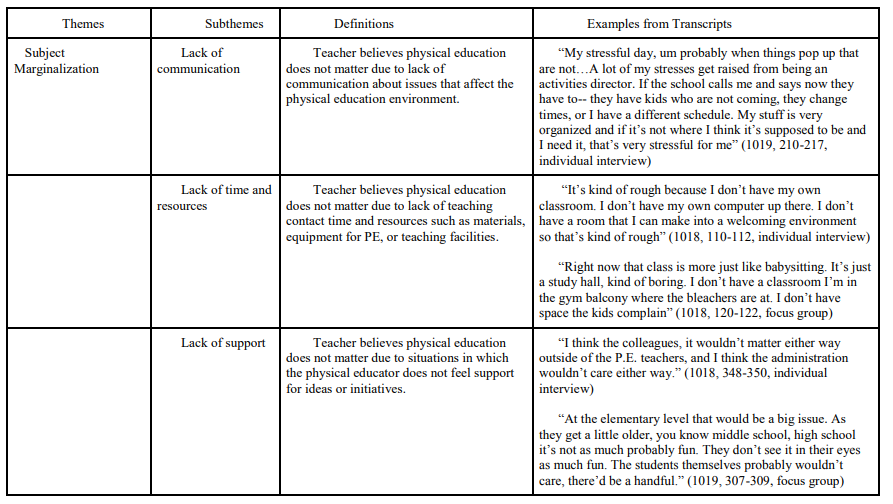
\includegraphics[width=\maxwidth{.95\linewidth}]{gfx/08-codebook}
	\caption{Example Codebook}
	\label{fig08.02}
\end{figure}

Data entry is the part of the survey where the data collected are entered into a computer for analysis. Most surveys are conducted online or using electronic devices like tablets so the data are already in digital format. It is also possible to use a data capture form that can be scanned into a computer. However, data that are collected using simple ``paper and pencil'' forms must be manually entered into a computer for analysis. This is a time consuming and, frankly, boring task that researchers must simply slog through before beginning analysis.

After the data are in a digital format then there are several good tools researchers can use for analysis. Quantitative data can be analyzed with \textit{R}, \textit{SPSS}, or \textit{Excel}. Of these tools, \textit{Excel} is the one most students are familiar with but its application for research statistical analysis is somewhat limited. \textit{SPSS} is very powerful but expensive. \textit{R} is available as a free download, is very powerful, but has a rather steep learning curve. 

Once the data are coded into a computer they must be analyzed. One of the simplest type of analysis is to look for patterns in the data. \Gls{univariate} analysis is the most basic form of quantitative analysis and involves finding patterns across just one variable. For \gls{continuousdata}, analysis tools include the central measure, histograms, and box plots. For \gls{discretedata}, analysis tools include frequency distributions and bar plots. \Gls{bivariate} analysis looks for relationships between two variables and analysis tools include correlations and scatter plots. Multivariate analysis looks for relationships between three or more variables. 

Another common method of data analysis is hypothesis testing. In this case, researchers have postulated a \gls{hypothesis} and then conduct research to either support or refute the hypothesis. Any of the pattern-finding tools mentioned in the previous paragraph can be used for hypothesis testing, but other more powerful tools are also available, like an \gls{anova} or Kruskal-Wallis H.

\subsection{Biases in Survey Research}

Despite all of its strengths and advantages, survey research is often tainted with systematic \glspl{bias} that may invalidate some of the inferences derived from such surveys. Five such biases are the non-response bias, sampling bias, social desirability bias, recall bias, and common method bias.

\begin{description}
	\item[Non-response bias]\label{08:nonresponse} Survey research is generally notorious for its low response rates. A response rate of $ 15-20\% $ is typical in a mail survey, even after two or three reminders. If the majority of the targeted respondents fail to respond to a survey, then a legitimate concern is whether non-respondents are not responding due to a systematic reason, which may raise questions about the validity of the study's results. For instance, dissatisfied customers tend to be more vocal about their experience than satisfied customers, and are therefore more likely to respond to questionnaire surveys or interview requests than satisfied customers. Hence, any respondent sample is likely to have a higher proportion of dissatisfied customers than the underlying population from which it is drawn. In this instance, not only will the results lack generalizability, but the observed outcomes may also be an artifact of the biased sample. The following strategies may be employed to improve response rates.

\begin{itemize}
	\item \textbf{Advance notification}. A short letter sent in advance to the targeted respondents soliciting their participation in an upcoming survey can prepare them in advance and improve their propensity to respond. The letter should state the purpose and importance of the study, mode of data collection (\eg, via a phone call, a survey form in the mail, etc.), and appreciation for their cooperation. A variation of this technique may request the respondent to return a postage-paid postcard indicating whether or not they are willing to participate in the study.

	\item \textbf{Relevance of content}. Respondents are more likely to respond to a survey that they consider relevant or important than to ones that do not matter.

	\item \textbf{Respondent-friendly questionnaire} Shorter survey questionnaires tend to elicit higher response rates than longer questionnaires. Furthermore, questions that are clear, non-offensive, and easy to respond to tend to attract higher response rates.

	\item \textbf{Endorsement}. For organizational surveys, it helps to gain the endorsement from a senior executive attesting to the importance of the study to the organization. Such endorsement can be in the form of a cover letter or a letter of introduction, which can improve the researcher's credibility in the eyes of the respondents.

	\item \textbf{Follow-up requests}. Multiple follow-up requests may coax some non-respondents to respond, even if their responses are late.

	\item \textbf{Interviewer training} Response rates for interviews can be improved with skilled interviewers trained on how to request interviews, use computerized dialing techniques to identify potential respondents, and schedule callbacks for respondents who could not be reached.

	\item \textbf{Incentives} Response rates, at least with certain populations, may increase with the use of incentives in the form of cash or gift cards, giveaways such as pens or stress balls, entry into a lottery, draw or contest, discount coupons, promise of contribution to charity, and so forth.

	\item \textbf{Non-monetary incentives} Businesses, in particular, are more prone to respond to non-monetary incentives than financial incentives. An example of such a non-monetary incentive is a bench marking report comparing the business's individual response against the aggregate of all responses to a survey.

	\item \textbf{Confidentiality and privacy}. Finally, assurances that the respondent's private data or responses will not fall into the hands of any third party may help improve response rates.
\end{itemize}

\item[Sampling bias] Bias can be introduced in a poorly-designed survey by using the wrong sample selection. Telephone surveys conducted by calling a random sample of publicly available mobile phone numbers will systematically exclude people with who do not own a mobile phone, and people who are unable to answer the phone (for instance, they are at work) when the survey is being conducted, and will include a disproportionate number of respondents who have who stay home during much of the day, such as the unemployed, the disabled, and the elderly. Likewise, online surveys tend to include a disproportionate number of students and younger people who are constantly on the Internet, and systematically exclude people with limited or no access to computers or the Internet, such as the poor and the elderly. Similarly, questionnaire surveys tend to exclude children and the illiterate, who are unable to read, understand, or meaningfully respond to the questionnaire. A different kind of sampling bias relate to sampling the wrong population, such as asking teachers (or parents) about academic learning of their students (or children), or asking CEOs about operational details in their company. Such biases make the respondent sample unrepresentative of the intended population and call into question generalizability claims about inferences drawn from the biased sample.

\item[Social desirability bias] Many respondents tend to avoid negative opinions or embarrassing comments about themselves, their employers, family, or friends. With negative questions such as ``do you think that your project team is dysfunctional,'' the researcher may not get truthful responses. This tendency among respondents to ``spin the truth'' in order to portray themselves in a socially desirable manner is called the ``social desirability bias,'' which hurts the validity of response obtained from survey research. There is practically no way of overcoming the social desirability bias in a questionnaire survey, but in an interview setting, an astute interviewer may be able to spot inconsistent answers and ask probing questions or use personal observations to supplement respondents' comments.

\item[Recall bias] Responses to survey questions often depend on subjects' motivation, memory, and ability to respond. Particularly when dealing with events that happened in the distant past, respondents may not adequately remember their own motivations or behaviors or perhaps their memory of such events may have evolved with time and no longer retrievable. For instance, if respondents are asked to describe their utilization of computer technology one year ago or even memorable childhood events like birthdays, their response may not be accurate due to difficulties with recall. One possible way of overcoming the recall bias is by anchoring respondent's memory in specific events as they happened, rather than asking them to recall their perceptions and motivations from memory.

\item[Common method bias] Common method bias refers to the amount of spurious covariance shared between independent and dependent variables that are measured at the same point in time, such as in a cross-sectional survey, using the same instrument, such as a questionnaire. In such cases, the phenomenon under investigation may not be adequately separated from measurement artifacts. This bias can be potentially avoided if the independent and dependent variables are measured at different points in time, using a longitudinal survey design, of if these variables are measured using different methods, such as computerized recording of dependent variable versus questionnaire-based self-rating of independent variables.

\end{description}

\section{Key Takeaways}

\begin{center}
	\begin{tkawybox}{Survey Research}
		\begin{itemize}
			\setlength{\itemsep}{0pt}
			\setlength{\parskip}{0pt}
			\setlength{\parsep}{0pt}
			
			\item Differentiate between cross-sectional and longitudinal surveys
			\item Compare and contrast the four types of longitudinal surveys: trend, panel, cohort, and retrospective
			\item Describe the characteristics of effective questions
			\item Define the various question response options
			\item Describe tips for creating good questionnaires
			\item Discuss how survey data are analyzed
			\item Discuss bias in survey research

		\end{itemize}
	\end{tkawybox}
\end{center}
